\documentclass[15pt]{standalone}
\usepackage{pgfplots}
\begin{document}
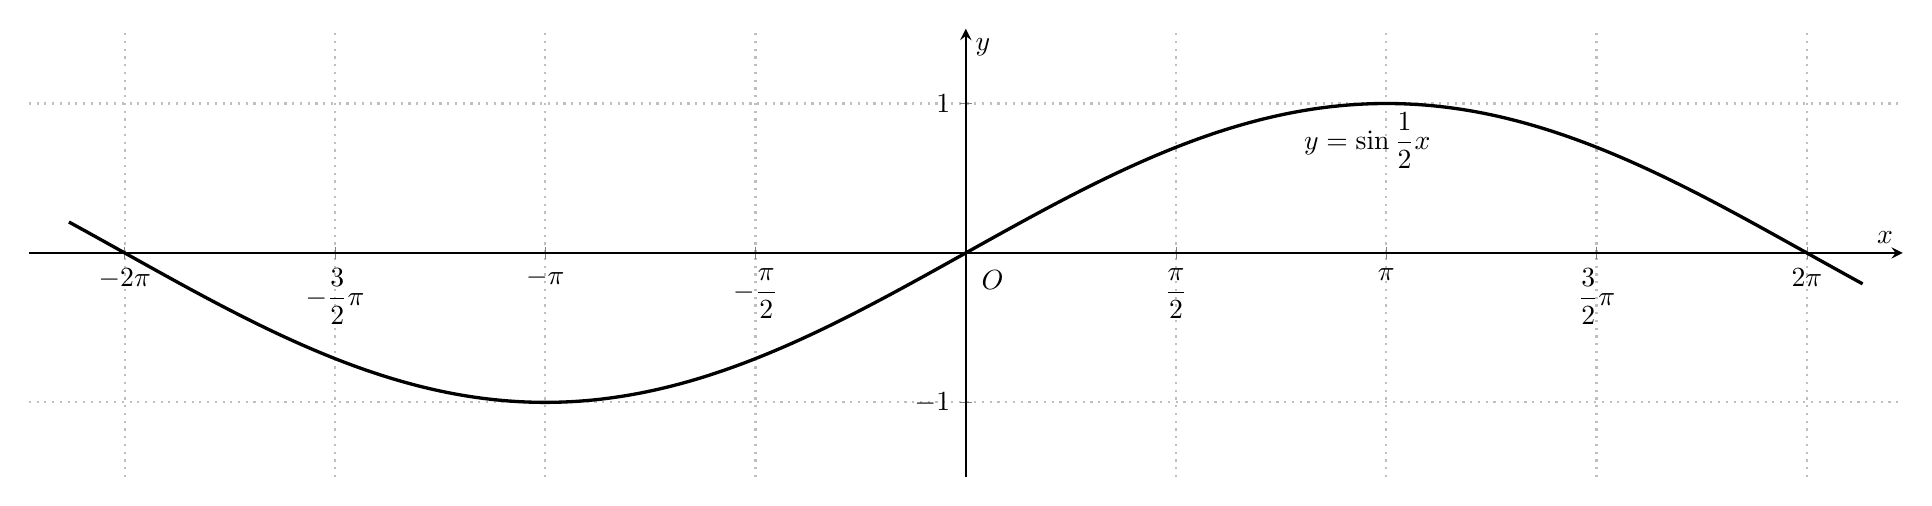
\begin{tikzpicture}
  \begin{axis}[
    axis lines=middle,
    axis line style=thick,
    grid=both,
    xmin=-7,
    xmax=7,
    ymax=1.5,
    ymin=-1.5,
    x=1.7cm,
    grid style={line width=.8pt, dotted},
    ytick={-1, 1},
    yticklabels={$-1$, $1$},
    xlabel=$x$,
    ylabel=$y$,
    xtick={%
      -2 * pi, -(3/2) * pi, -pi, -(1/2) * pi,
      (1/2) * pi, pi, (3/2) * pi, 2 * pi
    },
    xticklabels={%
      $-2 \pi$, $\displaystyle -\frac{3}{2}\pi$, $-\pi$, $\displaystyle -\frac{\pi}{2}$,
      $\displaystyle \frac{\pi}{2}$, $\pi$, $\displaystyle \frac{3}{2}\pi$, $2\pi$
    }
  ]
  \addplot[domain=-6.7:6.7, samples=200, smooth, very thick] {sin(deg(0.5 * x))};
  \node (O) at (axis cs:0.2, -0.18) {$O$};
  \node (O) at (axis cs:3, 0.75) {$\displaystyle y = \sin \frac{1}{2}x$};
  \end{axis}
\end{tikzpicture}
\end{document}
